\documentclass[12pt,titlepage]{article}
\usepackage[margin=1.25in]{geometry}
\usepackage{graphicx,amsmath,blindtext,minted}

%% Variables definition
\newcommand{\vSubject}{Data Structure and Algorithm Practicum}
\newcommand{\vSubtitle}{Double Linked Lists}
\newcommand{\vName}{Muhammad Baihaqi Aulia Asy'ari}
\newcommand{\vNIM}{2241720145}
\newcommand{\vClass}{1I}
\newcommand{\vDepartment}{Information Technology}
\newcommand{\vStudyProgram}{D4 Informatics Engineering}

%% [START] Tikz related stuff
\usepackage{tikz}
\usetikzlibrary{svg.path,calc,shapes.geometric,shapes.misc}
\tikzstyle{terminator} = [rectangle, draw, text centered, rounded corners = 1em, minimum height=2em]
\tikzstyle{preparation} = [chamfered rectangle, chamfered rectangle sep=0.75em, draw, text centered, minimum height = 2em]
\tikzstyle{process} = [rectangle, draw, text centered, minimum height=2em]
\tikzstyle{decision} = [diamond, aspect=2, draw, text centered, minimum height=2em]
\tikzstyle{data}=[trapezium, draw, text centered, trapezium left angle=60, trapezium right angle=120, minimum height=2em]
\tikzstyle{connector} = [line width=0.25mm,->]
%% [END] Tikz related stuff

%% [START] Fancy header related stuff
\usepackage{fancyhdr}
\pagestyle{fancy}
\setlength{\headheight}{15pt} % compensate fancyhdr style
\fancyhead{}
\fancyfoot{}
\fancyfoot[L]{\thepage}
\fancyfoot[R]{\textit{\vSubject - \vSubtitle}}
\renewcommand{\footrulewidth}{0.4pt}% default is 0pt, overline for footer
%% [END] Fancy header related stuff

%% [START] Custom tabular command related stuff
\usepackage{tabularx}
\newcommand{\details}[2]{
    #1 & #2  \\
}
%% [END] Custom tabular command related stuff

%% [START] Figure related stuff
\newcommand{\image}[3][1]{
    \begin{figure}[h]
        \centering
        \includegraphics[#1]{#2}
        \caption{#3}
        \label{#3}
    \end{figure}
}
%% [END] Figure related stuff

%%
\usepackage{pgf-umlcd}

\renewcommand{\umldrawcolor}{black}
\renewcommand{\umlfillcolor}{white}
%%

%% [BEGIN] Custom enumerator
\usepackage{enumitem}
%% [END] Custom enumerator

%% [BEGIN] Paragraph indent
\usepackage{indentfirst}
%% [END] Paragraph indent

\begin{document}
\begin{titlepage}
    \centering
    \vfill
    {\bfseries\LARGE
        \vSubject\\
        \vskip0.25cm
        \vSubtitle
    }
    \vfill
    
\includegraphics[width=6cm]{images/polinema-logo.png}
    \vfill
    {
        \textbf{Name}\\
        \vName\\
        \vskip0.5cm
        \textbf{NIM}\\
        \vNIM\\
        \vskip0.5cm
        \textbf{Class}\\
        \vClass\\
        \vskip0.5cm
        \textbf{Department}\\
        \vDepartment\\
        \vskip0.5cm
        \textbf{Study Program}\\
        \vStudyProgram
    }
\end{titlepage}

\newpage

\setcounter{section}{1}
\subsection{Learning Objective}
After learning this lab activity, students will be able to:
\begin{enumerate}
    \item Understand Double Linked List algorithm
    \item Create and declare double linked list algorithm
    \item Implement double linked list algorithm in various case studies
\end{enumerate}

\subsection{Lab Activities 1}
In this lab activity, we will create Node class and DoubleLinkedList class that has operations to insert data in multiple way. (from the beginning or the tail of the list)

\subsubsection{Steps}
\begin{enumerate}
    \item Take this class diagram as your reference for creating the \textbf{DoubleLinkedList class}
    \mbox{}\\
    \mbox{}\\
    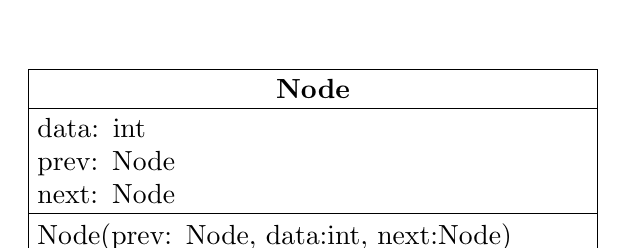
\begin{tikzpicture}
        \begin{class}[text width=7cm]{Node}{0,0}
            \attribute{data: int}
            \attribute{prev: Node}
            \attribute{next: Node}
            \operation{Node(prev: Node, data:int, next:Node)}
        \end{class}
    \end{tikzpicture}
    \mbox{}\\
    \mbox{}\\
    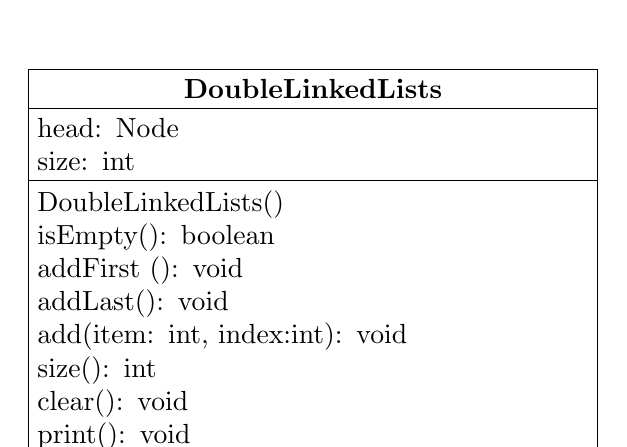
\begin{tikzpicture}
        \begin{class}[text width=7cm]{DoubleLinkedLists}{0,0}
            \attribute{head: Node}
            \attribute{size: int}
            \operation{DoubleLinkedLists()}
            \operation{isEmpty(): boolean}
            \operation{addFirst (): void}
            \operation{addLast(): void}
            \operation{add(item: int, index:int): void}
            \operation{size(): int}
            \operation{clear(): void}
            \operation{print(): void}
        \end{class}
    \end{tikzpicture}
    \mbox{}\\
    \item Create a new package named \textbf{DoubleLinkedList}
    \item Create a new class in that package named \textbf{Node}
    \item In that class, declare the attributes as described in the class diagram
    \begin{minted}[autogobble,breaklines]{java}
        int data;
        Node prev, next;
    \end{minted}
    \item Next, add the default constructor in Node class
    \begin{minted}[autogobble,breaklines]{java}
        public Node(Node prev, int data, Node next) {
            this.data = data;
            this.prev = prev;
            this.next = next;
        }
    \end{minted}
    \item Create a new class named \textbf{DoubleLinkedList} in the same package with the node as following image:
    \begin{minted}[autogobble,breaklines]{java}
        package LabActivities;

        public class DoubleLinkedList {
        
        }
    \end{minted}
    \item Next, we add the attributes
    \begin{minted}[autogobble,breaklines]{java}
        Node head;
        int size;
    \end{minted}
    \item Then, add the constructor in class \textbf{DoubleLinkedList}
    \begin{minted}[autogobble,breaklines]{java}
        public DoubleLinkedList() {
            head = null;
            size = 0;
        }
    \end{minted}
    \item Create method isEmpty(), this method will be used to check whether the linked list is empty or not
    \begin{minted}[autogobble,breaklines]{java}
        public boolean isEmpty() {
            return head == null;
        }
    \end{minted}
    \item Then add method \textbf{addFirst()}. This method will be executed when we want to add data in the beginning of the list
    \begin{minted}[autogobble,breaklines]{java}
        public void addFirst(int item) {
            if (isEmpty()) {
                head = new Node(null, item, null);
            } else {
                Node newNode = new Node(null, item, head);
                head.prev = newNode;
                head = newNode;
            }
            size++;
        }
    \end{minted}
    \item Let’s not forget about adding the data in the end of the list. We can do it after adding these lines of code in \textbf{addLast()} method
    \begin{minted}[autogobble,breaklines]{java}
        public void addLast(int item) {
            if (isEmpty()) {
                addFirst(item);
            } else {
                Node current = head;
                while (current.next != null) {
                    current = current.next;
                }
                Node newNode = new Node(current, item, null);
                current.next = newNode;
                size++;
            }
        }
    \end{minted}
    \item If we want to add a data that specified by a certain index, we will need to provide additional method to do so. It can be done by creating the \textbf{add()} method
    \begin{minted}[autogobble,breaklines]{java}
        public void add(int item, int index) throws Exception{
            if (isEmpty()) {
                addFirst(item);
            } else if (index < 0 || index > size) {
                throw new Exception("Index out of bound");
            } else {
                Node current = head;
                int i = 0;
                while (i < index) {
                    current = current.next;
                    i++;
                }
                if (current.next == null) {
                    Node newNode = new Node(null, item, current);
                    current.prev = newNode;
                    head = newNode;
                } else {
                    Node newNode = new Node(current.prev, item, current);
                    newNode.prev = current.prev;
                    newNode.next = current;
                    current.prev.next = newNode;
                    current.prev = newNode;
                }
            }
            size++;
        }
    \end{minted}
    \item We want to make our list has an easy access to retrieve the length of the list. That’s why we create method \textbf{size()}
    \begin{minted}[autogobble,breaklines]{java}
        public int size() {
            return size;
        }
    \end{minted}
    \item We create a method \textbf{clear()} to remove all the data that are exist in linked lists
    \begin{minted}[autogobble,breaklines]{java}
        public void clear() {
            head = null;
            size = 0;
        }
    \end{minted}
    \item Next up, to print the whole data in the list, we need to create a method print().
    \begin{minted}[autogobble,breaklines]{java}
        public void print() {
            if (!isEmpty()) {
                Node temp = head;
                while (temp != null) {
                    System.out.print(temp.data + "\t");
                    temp = temp.next;
                }
                System.out.println("\n successfully added");
            } else {
                System.out.println("Linked list is empty");
            }
        }
    \end{minted}
    \item After creating the blueprint classes, we will need one main class so that all of that can be included in the program. Create \textbf{DoubleLinkedListMain} class to do so
    \begin{minted}[autogobble,breaklines]{java}
        package LabActivities;

        public class DoubleLinkedListMain {
            public static void main(String[] args) throws Exception {

            }
        }
    \end{minted}
    \item Instantiate an object from \textbf{DoubleLinkedList} class in the main method. Then apply these program code
    \begin{minted}[autogobble,breaklines]{java}
        DoubleLinkedList dll = new DoubleLinkedList();
        dll.print();
        System.out.println("Size: " + dll.size);
        System.out.println("================================================");
        dll.addFirst(3);
        dll.addLast(4);
        dll.addFirst(7);
        dll.print();
        System.out.println("Size: " + dll.size);
        System.out.println("================================================");
        dll.add(40, 1);
        dll.print();
        System.out.println("Size: " + dll.size);
        System.out.println("================================================");
        dll.clear();
        dll.print();
        System.out.println("Size: " + dll.size);
    \end{minted}
\end{enumerate}

\subsubsection{Result}
Compile the program and see if the result matches with following image
\begin{minted}[autogobble,breaklines,linenos]{text}
    PS D:\Kuliah\Smt 2\Algoritma dan Struktur Data\Praktikum\Week 12\Double Linked Lists>  d:; cd 'd:\Kuliah\Smt 2\Algoritma dan Struktur Data\Praktikum\Week 12\Double Linked Lists'; & 'C:\Program Files\Java\jdk-18.0.2.1\bin\java.exe' '-XX:+ShowCodeDetailsInExceptionMessages' '-cp' 'D:\Kuliah\Smt 2\Algoritma dan Struktur Data\Praktikum\Week 12\Double Linked Lists\bin' 'LabActivities.DoubleLinkedListMain'
    Linked list is empty
    Size: 0
    ================================================
    7       3       4
    successfully added
    Size: 3
    ================================================
    7       40      3       4
    successfully added
    Size: 4
    ================================================
    Linked list is empty
    Size: 0
\end{minted}

\subsubsection{Questions}
\begin{enumerate}
    \item What’s the difference between single linked list and double linked list?
    \item In \textbf{Node class}, what is the usage of attribute next and prev ?
    \item In constructor of \textbf{DoubleLinkedList} class. What’s the purpose of head and size attribute
    in this following code?
    \item In method \textbf{addFirst()}, why do we initialize the value of Node object to be null at first?
    Node newNode = new Node(null, item, head);
    \item In method \textbf{addLast()}, what’s the purpose of creating a node object by passing the \textbf{prev} parameter with \textbf{current} and \textbf{next} with \textbf{null} ?
    Node newNode = new Node(current, item, null);
\end{enumerate}

\subsection{Lab Activities 2}
In this lab activity, we have added some methods from our 1\textsuperscript{st} lab activity. Now, we added some ways for the users to remove a data in the beginning of the list, the tail, or with specified index. For more details, pay attention to this class diagram:
\mbox{}\\
\mbox{}\\
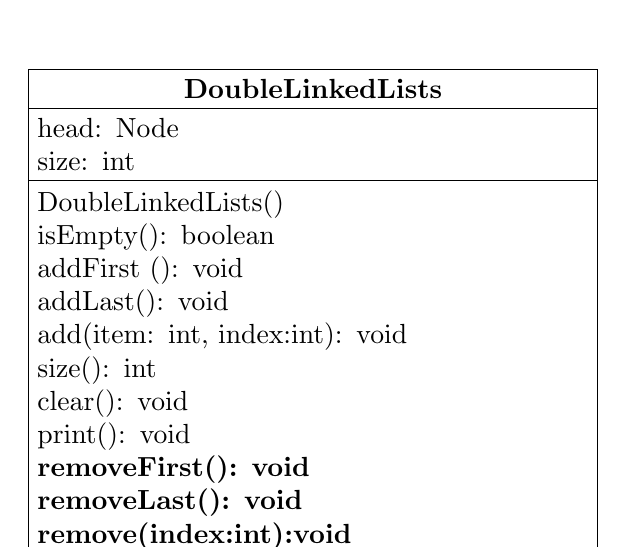
\begin{tikzpicture}
    \begin{class}[text width=7cm]{DoubleLinkedLists}{0,0}
        \attribute{head: Node}
        \attribute{size: int}
        \operation{DoubleLinkedLists()}
        \operation{isEmpty(): boolean}
        \operation{addFirst (): void}
        \operation{addLast(): void}
        \operation{add(item: int, index:int): void}
        \operation{size(): int}
        \operation{clear(): void}
        \operation{print(): void}
        \operation{ \textbf{removeFirst(): void}}
        \operation{ \textbf{removeLast(): void}}
        \operation{ \textbf{remove(index:int):void}}
    \end{class}
\end{tikzpicture}
\mbox{}\\

\subsubsection{Steps}
\begin{enumerate}
    \item Create method \textbf{removeFirst()} in class \textbf{DoubleLinkedList}
    \begin{minted}[autogobble,breaklines]{java}
        public void removeFirst() throws Exception{
            if (isEmpty()) {
                throw new Exception("Linked list is still empty, cannot remove data");
            } else if (size == 1) {
                removeLast();
            } else {
                head = head.next;
                head.prev = null;
                size--;
            }
        }
    \end{minted}
    \item Create method \textbf{removeLast()} in class \textbf{DoubleLinkedList}
    \begin{minted}[autogobble,breaklines]{java}
        public void removeLast() throws Exception{
            if (isEmpty()) {
                throw new Exception("Linked list is still empty, cannot remove data");
            } else if (head.next == null) {
                head = null;
                size--;
                return;
            } 
            Node current = head;
            while (current.next.next != null) {
                current = current.next;
            }
            current.next = null;
            size--;
        }
    \end{minted}
    \item Create method \textbf{remove()} in class \textbf{DoubleLinkedList}, alongside with its parameter
    \begin{minted}[autogobble,breaklines]{java}
        public void remove(int index) throws Exception{
            if (isEmpty() || index >= size) {
                throw new Exception("Index value is out of bound");
            } else if (size == 0) {
                removeFirst();
            } else {
                Node current = head;
                int i = 0;
                while (i < index) {
                    current = current.next;
                    i++;
                }
                if (current.next == null) {
                    current.prev.next = null;
                } else if (current.prev == null) {
                    current = current.next;
                    current.prev = null;
                    head = current;
                } else {
                    current.prev.next = current.next;
                    current.next.prev = current.prev;
                }
                size--;
            }
        }
    \end{minted}
    \item To execute additional codes we’ve just added, also make addition in the main class as well
    \begin{minted}[autogobble,breaklines]{java}
        dll.addLast(50);
        dll.addLast(40);
        dll.addLast(10);
        dll.addLast(20);
        dll.print();
        System.out.println("Size: " + dll.size);
        System.out.println("================================================");
        dll.removeFirst();
        dll.print();
        System.out.println("Size: " + dll.size);
        System.out.println("================================================");
        dll.removeLast();
        dll.print();
        System.out.println("Size: " + dll.size);
        System.out.println("================================================");
        dll.remove(1);
        dll.print();
        System.out.println("Size: " + dll.size);
    \end{minted}
\end{enumerate}

\subsubsection{Result}
Compile the program and see if the result matches with following image
\begin{minted}[autogobble,breaklines,linenos]{text}
    PS D:\Kuliah\Smt 2\Algoritma dan Struktur Data\Praktikum\Week 12\Double Linked Lists>  d:; cd 'd:\Kuliah\Smt 2\Algoritma dan Struktur Data\Praktikum\Week 12\Double Linked Lists'; & 'C:\Program Files\Java\jdk-18.0.2.1\bin\java.exe' '-XX:+ShowCodeDetailsInExceptionMessages' '-cp' 'D:\Kuliah\Smt 2\Algoritma dan Struktur Data\Praktikum\Week 12\Double Linked Lists\bin' 'LabActivities.DoubleLinkedListMain' 
    50      40      10      20
    successfully added
    Size: 4
    ================================================
    40      10      20
    successfully added
    Size: 3
    ================================================
    40      10
    successfully added
    Size: 2
    ================================================
    40
    successfully added
    Size: 1
\end{minted}

\subsubsection{Questions}
\begin{enumerate}
    \item What’s the meaning of these statements in \textbf{removeFirst()} method?
    \item How do we detect the position of the data that are in the last index in method \textbf{removeLast()}?
    \item Explain why this program code is not suitable if we include it in \textbf{remove} command!
    \item Explain what’s the function of this program code in method \textbf{remove}!
\end{enumerate}

\subsection{Lab Activities 3}
In this 3\textsuperscript{rd} lab activity, we will test if we can retrieve a data in linked list in various needs. The first is we can get a data in the beginning of the list, at the end of the list, or in specified index of the list. We will create 3 methods to realize the idea. For more details, feel free to check this class diagram
\mbox{}\\
\mbox{}\\
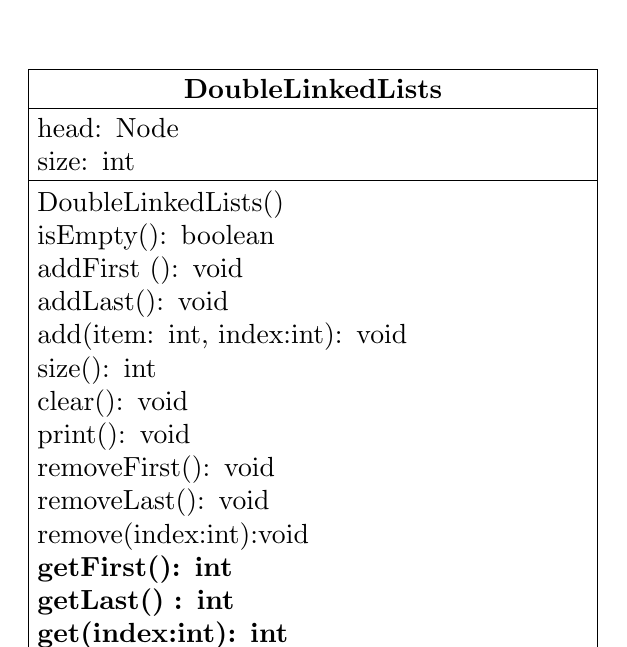
\begin{tikzpicture}
    \begin{class}[text width=7cm]{DoubleLinkedLists}{0,0}
        \attribute{head: Node}
        \attribute{size: int}
        \operation{DoubleLinkedLists()}
        \operation{isEmpty(): boolean}
        \operation{addFirst (): void}
        \operation{addLast(): void}
        \operation{add(item: int, index:int): void}
        \operation{size(): int}
        \operation{clear(): void}
        \operation{print(): void}
        \operation{removeFirst(): void}
        \operation{removeLast(): void}
        \operation{remove(index:int):void}
        \operation{ \textbf{getFirst(): int}}
        \operation{ \textbf{getLast() : int}}
        \operation{ \textbf{get(index:int): int}}
    \end{class}
\end{tikzpicture}
\mbox{}\\

\subsubsection{Steps}
\begin{enumerate}
    \item Create a method \textbf{getFirst()} in class \textbf{DoubleLinkedList} to retrieve the first data in the list
    \begin{minted}[autogobble,breaklines]{java}
        public int getFirst() throws Exception{
            if (isEmpty()) {
                throw new Exception("Linked list still empty");
            }
            return head.data;
        }
    \end{minted}
    \item Create a method \textbf{getLast()} in class \textbf{DoubleLinkedList} to retrieve the data in the list
    \begin{minted}[autogobble,breaklines]{java}
        public int getLast() throws Exception{
            if (isEmpty()) {
                throw new Exception("Linked list still empty");
            }
            Node temp = head;
            while (temp.next != null) {
                temp = temp.next;
            }
            return temp.data;
        }
    \end{minted}
    \item Create a method \textbf{get(int index)} in class \textbf{DoubleLinkedList} to retrieve the data in specified index of the list
    \begin{minted}[autogobble,breaklines]{java}
        public int get(int index) throws Exception{
            if (isEmpty()) {
                throw new Exception("Linked list still empty");
            }
            Node temp = head;
            for (int i = 0; i < index; i++) {
                temp = temp.next;
            }
            return temp.data;
        }
    \end{minted}
    \item In the main class, add the program code as follows and see the result
    \begin{minted}[autogobble,breaklines]{java}
        dll.print();
        System.out.println("Size: " + dll.size);
        System.out.println("================================================");
        dll.addFirst(3);
        dll.addLast(4);
        dll.addFirst(7);
        dll.print();
        System.out.println("Size: " + dll.size);
        System.out.println("================================================");

        dll.add(40,1);
        dll.print();

        System.out.println("Size: " + dll.size);
        System.out.println("================================================");
        System.out.println("Data in the head of the linked list is : " + dll.getFirst());
        System.out.println("Data in the tail of the linked list is : " + dll.getLast());
        System.out.println("Data in the 1st index of the linked list is : " + dll.get(1));
    \end{minted}
\end{enumerate}

\subsubsection{Result}
Compile the program and see if the result matches with following image
\begin{minted}[autogobble,breaklines,linenos]{text}
    PS D:\Kuliah\Smt 2\Algoritma dan Struktur Data\Praktikum\Week 12\Double Linked Lists>  d:; cd 'd:\Kuliah\Smt 2\Algoritma dan Struktur Data\Praktikum\Week 12\Double Linked Lists'; & 'C:\Program Files\Java\jdk-18.0.2.1\bin\java.exe' '-XX:+ShowCodeDetailsInExceptionMessages' '-cp' 'D:\Kuliah\Smt 2\Algoritma dan Struktur Data\Praktikum\Week 12\Double Linked Lists\bin' 'LabActivities.DoubleLinkedListMain' 
    Linked list is empty
    Size: 0
    ================================================
    7       3       4
    successfully added
    Size: 3
    ================================================
    7       40      3       4
    successfully added
    Size: 4
    ================================================
    Data in the head of the linked list is : 7
    Data in the tail of the linked list is : 4
    Data in the 1st index of the linked list is : 40
\end{minted}

\subsubsection{Questions}
\begin{enumerate}
    \item What is the function of method \textbf{size()} in \textbf{DoubleLinkedList} class ?
    \item How do we set the index in double linked list so that it starts from 1st index instead of 0th index?
    \item Please explain the difference between method \textbf{Add()} in double linked list and single linked list !
    \item What’s the logic difference of these 2 following codes?
\end{enumerate}

\subsection{Assignment}
\begin{enumerate} 
    \item Create a program with double linked list implementation that allows user to choose a menu as following image! The searching uses sequential search approach and the program should be able to sort the data in descending order. You may any choose sorting approach you prefer (bubble sort, selection sort, insertion sort, or merge sort)
    \hbox{}\\\textbf{Adding a data}
    \hbox{}\\\textbf{Add data in specified index and display the result}
    \hbox{}\\\textbf{Search Data}
    \hbox{}\\\textbf{Sorting Data}
    \item We are required to create a program which Implement Stack using double linked list. The features are described in following illustrations:
    \hbox{}\\\textbf{Initial menu and add Data (push)}
    \hbox{}\\\textbf{Print All Data}
    \hbox{}\\\textbf{See the data on top of the stack}
    \hbox{}\\\textbf{Pop the data from the top of the stack}
    \item Create a program that helps vaccination process by having a queue algorithm alongside with double linked list as follows \textbf{(the amount left of queue length in menu print(3) and recent vaccinated person in menu Remove data (2) should be displayed)}
    \hbox{}\\\textbf{Initial menu and adding a data}
    \hbox{}\\\textbf{Print data (notice the highlighted red in the result)}
    \hbox{}\\\textbf{Remove Data (the highlighted red must displayed in the console too)}
    \item Create a program implementation that list students score. Each student’s data consist of their nim, name, and gpa. The program should implement double linked list and should be able to search based on NIM and sort the GPA in descending order. \textbf{Students class must be implemented in this program}
    \hbox{}\\\textbf{Initial menu and adding data}
    \hbox{}\\\textbf{Printing data}
    \hbox{}\\\textbf{Searching data}
    \hbox{}\\\textbf{Sorting data}
\end{enumerate}

\end{document}